\documentclass{acm_proc_article-sp}

\usepackage{amsmath,amssymb}
\usepackage{latexsym}
\usepackage{indentfirst}
\usepackage{blindtext}
\usepackage{graphicx}
\usepackage{caption}
\usepackage{subcaption}
\usepackage{url}

\DeclareMathOperator*{\argmax}{arg\,max}
\DeclareMathOperator*{\minbelow}{min}

\begin{document}

\title{Object Tracking}
\subtitle{A Quantitative Comparison}
\author{Chuhang Zou, Zheng Yan, Yi Shi, Qing Ren, Caihua Shan, Jueji Yang}
\maketitle

\begin{abstract}
Object tracking is a such import task in computer vision that many kinds of methods are developed to solve this problem. Most of these methods have released their codes and datasets on the Internet. It is meaningful to evaluate these methods with unified criteria. We will briefly introduce these algorithms and then pick some datasets from Internet to test all the algorithms on some criterion to see their performance and make an advise about what kind of image sequence each algorithm is better for.
\end{abstract}

\section{Introduction}
Object tracking is one of the core problems in a wide range of applications in computer vision, such as surveillance, human computer interaction, augmented reality, and medical imaging.
In most areas of computer vision like scene understanding and action recognition, object tracking is regarded as an essential component.
Object tracking problem is to estimate the position of target in video sequence given the position of the target in the first frame.
Lots of algorithms and studies have been established to solve object tracking problem in the recent years.
But most algorithms perform bad when occlusion or out-of-view appears in the sequence.
Therefore, we evaluate the performance over the data sequence separately and discuss the bad cases for each algorithm.

The input data of object tracking problem can be image sequence or videos.
The predict position of the target in a frame is rectangle which can be 2 diagonal angles or 1 angle with width and height.
It needs lots of human effort to sample images using camera and label the position of the target by our own.
And the content of the images are not rich, most of which will be our faces.
Thus, we collect our data from the Internet\cite{dataset}.
These datas contain out-of-view, occlusion, illumination variation, scale variation, deformation, motion blur, fast motion, background clutters and other factors that will cause large tracking inaccuracy which is rich enough to test these state-of-art algorithms.

There are large mount of algorithms released to the public including Struck\cite{struck}, deep learning track\cite{dlt}, DFT\cite{dcmt}, ASLA\cite{asla}, TLD\cite{tld}, CXT\cite{cxt} and other state-of-art methods that perform quite well in their papers. 
We find these methods have mainly two problems: 
1). Overfitting on the initial frame with initial position, which will cause target missing when occlusion, out-of-plane rotation happen, but perform better in fast motion and out-of-view situations;
2). Online training over the sequence and overfitting the following tracked images will cause target shift when out-of-view happened.
To test the algorithms on these two problems, we pick out some notable image sequences, and discuss the performance of each algorithm to see whether the two problems happened on them.

\section{Related Work}
In this section, we review recent algorithms related to the six methods we chosen.
These methods are based on quite different modules so there is much related work.
Due to limitations on space, we just choose the important based work of each method.

DFT uses mixed discrete-continuous formulation to describe the situation: data association between target detections and trajectories is kept discrete, nonetheless trajectory fitting is performed in the continuous domain.
In contrast to previous discrete-continuous approaches based on Markov Chain Monte Carlo (MCMC) sampling\cite{rw4}\cite{rw5}, the data association continues to be amenable to well-established discrete optimization techniques for labeling problems, such as graph cuts\cite{rw2}\cite{rw3} and (tree-reweighted) belief propagation\cite{rw1}.

DLT attempts to combine the philosophies behind both generative and discriminative trackers by developing a robust discriminative tracker which uses an effective image representation learned automatically.
Some popular generative trackers include incremental visual tracking (IVT), which represents the tracked object based on principal component analysis (PCA), and the l1 tracker (L1T).
Some representative trackers in this category are the online AdaBoost (OAB) tracker, multiple instance learning (MIL) tracker, and structured output tracker.

ASLA bears some similarity to\cite{rw6} in the use of local sparse representations.
However, it samples larger overlapped local image patches with fixed spatial layout where there are more spatial structural information in them.

CXT builds on P-N learning\cite{rw7}. 
Basically it inherits the power of tracking-learning-detection (TLD)\cite{rw8} framework while focusing on exploring the structure of unlabeled data.
To address the issue that it's vulnerable to switching to another similar object, it proposes to employ the tracking-learning-detection concept of this tracker to not only explore the structure of positive and negative data but also the more semantic data: Distracters and Supporters.

Struck makes use of the structured output SVM framework of\cite{rw9} because of this flexibility of SVMs and their natural generalization to structured output spaces.
In particular, we extend the online structured output SVM learning method proposed in\cite{rw10}\cite{rw11} and adapt it to the tracking problem.

\section{Evaluated Algorithms}
In this report, we investigate 6 visual tracking works and search for an appropriate evaluation criteria for those work. The algorithm details of these 6 tracking methods are listed as follow:

\subsection{Struck}
Struck\cite{struck} is different from other tracking-by-detection algorithms. Struck learns a function that directly estimates the object transformation between frames. Discriminant function $F:\mathcal{X} \times \mathcal{Y} \to \mathcal{R}$ with $X$ the sequence of images and $Y$ the possible bounding boxes transformations is used to predict:
\[
y_t = f(x_t^{P_{t-1}}) = \argmax_{y\in \mathcal{Y}}F(x_t^{P_{t-1}},y)
\]
where $t$ is time. $x_t^{P_{t-1}}$is the image with estimated bounding box at time $t-1$ and image pixels at time $t$. $F$ measures the compatibility between $(x,y)$ pairs, when $x$ and $y$ are well matched, $F$ gives a high score:
\[
F(x,y)=\langle w, \Phi(x,y) \rangle
\]
The parameter $w$ can be optimized by:
\begin{align}
\minbelow_w	&\frac{1}{2}||w||^2 + C \sum_{i=1}^n\xi_i\nonumber\\
	s.t.	&\forall i: \xi_i \ge 0\nonumber\\
			&\forall i, \forall y\not= y_i : \langle w, \delta\Phi_i(y)\rangle \ge \Delta(y_i,y)-\xi_i
\end{align}
$\delta\Phi_i(y)=\Phi(x_i, y_i) - \Phi(x_i, y)$. This optimization aims to ensure that the value of $F(x_i, y_i)$ is greater than $F(x_i, y)$ for $y\not= y_i$. $1-\Delta(y,\bar{y})$ is the bounding box overlap between $y$ and $\bar{y}$.

The paper optimize the dual form of the optimization which will not be listed here in detail. $\Phi(x,y)$ only appears in inner products in the dual form of this optimization. So a joint kernel function $k(x,y,\bar{x},\bar{y}) = \langle \Phi(x,y), \Phi(\bar{x},\bar{y})\rangle$ is used which is the kernel between features(Haar, Histogram) of cropped boxes of images. And SMO-style step is also used to optimize the dual secondary convex optimization.

\subsection{The Deep Learning Tracker}
According to \cite{dlt}, they propose a novel deep learning tracker (DLT) for robust visual tracking.

During the offline training stage, they train an large stacked denoising autoencoder (SDAE) containing five small denoising autoencoders (DAEs) with the Tiny Images dataset \cite{tiny} as auxiliary image data to learn generic natural image features.
We show the architecture of DAE and the whole structure of the SDAE in Fig.~\ref{fig:dlt}(a) and Fig.~\ref{fig:dlt}(b) respectively.

During the online tracking process, an additional classification layer is added to the encoder part of the trained SDAE to result in a classification neural network.
The object to track is specified by the location of its bounding box in the first frame as a positive example.
Some negative examples are collected from the background at a short distance from the object in order to fine-tune the classification layer.
The whole network can be tuned in many times during the entire tracking process.
The overall network architecture is shown in Fig.~\ref{fig:dlt}(c).

\begin{center}
    \begin{figure}[hbt]
      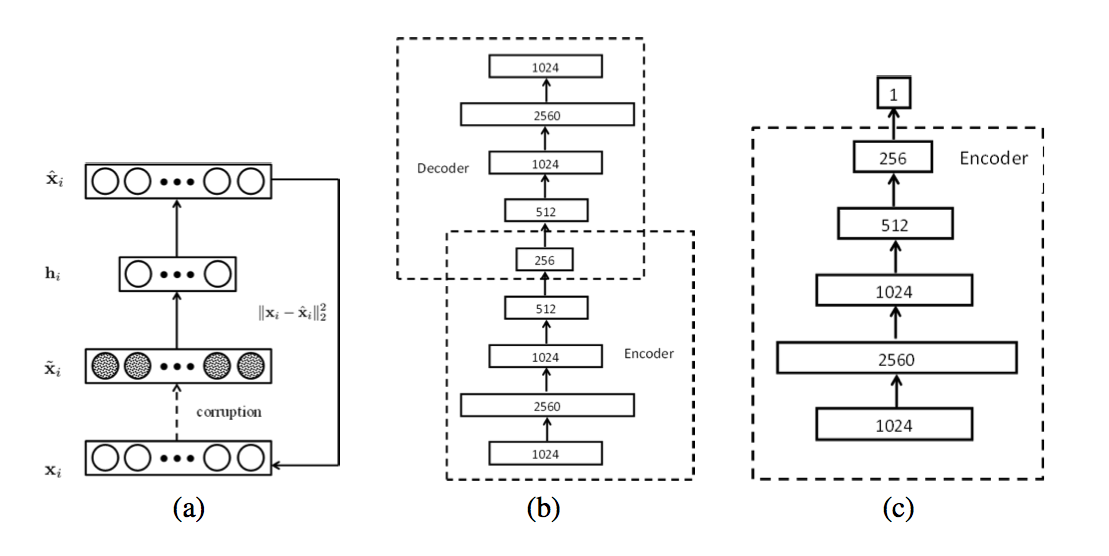
\includegraphics[width=0.5\textwidth]{dlt.png}
      \caption{Some key components of the network architecture: (a) denoising autoencoder; (b) stacked denoising autoencoder; (c) network for online tracking.}
      \label{fig:dlt}
    \end{figure}
\end{center}

\subsection{Context Tracker}
    CXT(Context Tracker) uses additional context information to build a strong model. It uses two different terms: 1) Distracters are regions that have similar appearance as the target, 2) Supporters are local key-points around the object having motion correlation with the target in a short time span. The goal of this algorithm is to find all possible regions which look similar to the target to prevent drift, and to look for useful information around the target to have strong verification.
    
    The paper uses P-N Tracker as the basic target tracker with several extensions. It extends the randomized ferns to accept multiple objects, applies 6bitBP which helps to boost up the speed of the detector and uses online template-based object model by constructing it in binary search tree using k-means.
    \newline
    As for distracters, a testing sample confidence score is computed using Normalized Cross-Correlation(NCC) between it and the closest image patch in the object model. It chooses the best candidate as the tracking result and the remaining regions trigger new distracter trackers.
    \newline
    Assuming that there are the valid target at frame t, the supporters are extracted around the location of that target with a radius R.
    \newline
    In unconstrained environments, the target may leave the FoV, or be completely occluded by other objects. The common trackers will simply switch to another region satisfying the threshold. Here, this tracker automatically exploits all the distracters and pays attention to them by tracking them simultaneously. Also, this tracker discovers a set of supporters to robustly identify the target among other similar regions.

\subsection{ASLA}

\label{sec:asla_section}

Visual Tracking via Adaptive Structural Local Sparse Appearance Model (ASLA) is one of Posters in CVPR2012 and performs favorably against several state-of-the-art methods on benchmark challenge.

ASLA is an efficient methods combined with structural local sparse model and adaptive template update strategy. It samples overlapped local image patches within the target region, whose sparse coding obtained by a novel alignment-pooling method contains both spatial and partial information of the target object. This representation guarantees more accurately location and less occlusion drift. In addition, the online adaptive template strategy based on both incremental subspace learning and sparse representation is employed in coding, far more improving the performance compared by methods based on static local or holistic sparse dictionary when there is similar object in the scenes.

The proposed algorithm is implemented in MATLAB and runs at 1.5 frames per second on a Pentium 2.7 GHz Dual Core PC with 2GB memory.

The $l_1$ minimization problem is solved with the SPAMS package and the regularization constant $\lambda$ is set to 0.01 in all experiments. For each sequence, the location of the target object is manually labeled in the first frame. We resize the target image patch to $32\times 32$ pixels and extract overlapped $16\times16$ local patches within the target region with 8 pixels as step length. As for the template update, 8 eigenvectors are used to carry out incremental subspace learning method in all experiments every 5 frames.

\subsection{TLD}
TLD proposes a new paradigm for learning from structured unlabeled data. The structure in the data is exploited by so called positive and negative structural constraints, which enforce certain labeling of the unlabeled set. Positive constraints specify the acceptable patterns of positive labels, i.e. patches close to the object trajectory are positive. Negative constraints specify acceptable patterns of negative labels, i.e. surrounding of the trajectory is negative. These constrains are used in parallel and we show that their combination enables mutual compensation of their errors. These constraints operate on the whole unlabeled set and therefore exploit different source of information than the classifier which operates on single examples only.

The availability of a small number of labeled examples and a large number of structured unlabeled examples suggest the following learning strategy: (i) Using the labeled samples, train an initial classifier and adjust the predefined constraints with the labeled data. (ii) Label the unlabeled data by the classifier and identify examples which have been labeled in contradiction with the structural constraints. (iii) Correct their labels, add to the training set and retrain the classifier. We call this bootstrapping process P-N learning.

The contribution of the TLD is a formalization of the P-N learning paradigm for off-line and on-line learning problems. TLD is processing the video sequence in real-time and the resulting detector achieves state-of-the-art performance.

\subsection{Distribution Fields for Tracking}
Visual tracking of general objects often relies on the assumption that gradient descent of the
alignment function will reach the global optimum. A common technique to smooth the objective function is to blur the image. However, blurring the image destroys image information, which can cause the target to be lost. To address this problem the author introduce a method for building an image descriptor using distribution fields (DFs), a representation that allows smoothing the objective function without destroying information about pixel values. They present experimental evidence on the superiority of the width of the basin of attraction around the global optimum of DFs over other descriptors. DFs also allow the representation of uncertainty about the tracked object. This helps in disregarding outliers during tracking (like occlusions or small misalignments) without modeling them explicitly.

\section{Evaluation Criterion}

In this report, we use success plot for quantitative analysis.
In addition, we evaluate speed of each algorithm by average running time in fps.

\textbf{Success plot.}
One widely used evaluation metric on tracking precision is the bounding box overlap. 
Given the tracked bounding box $r_t$ and the ground truth bounding box $r_a$, the overlap score is defined as $S = \frac{|r_t \bigcap r_a|}{|r_t \bigcup r_a|}$.
And then calculate the percentage of frames that has a score bigger than overlap threshold showed in Fig.~\ref{fig:soccer}.
The success plot shows the ratios of successful frames at the thresholds varied from 0 to 1. 

\textbf{Average running time.}
Average running time is a metric which can judge whether the algorithm is sufficient for real-time applications.
We represent average running time in fps to give readers a more direct sense.


\section{Experiments}

We choose 10 image sequences from website \cite{dataset} to cover all situations.
For each tracker, we fine-tuned parameters in the source code by our hand for each sequences to show the best of each algorithms. Then we show how each algorithms performs, and analysis why it is good or bad. What's more, we compute the average running time of each algorithms to analysis whether it is sufficient for real-time applications. 

\subsection{Sequences Analysis}

The performance in each sequence for all the trackers is summarized by the success plots as shown in Fig~\ref{fig:soccer} to Fig~\ref{fig:woman}.

Struck detects 9 frames per second with budget size of 100 and Haar feature.
In these ten image sequence, truck performs not good in Soccer and SUV.
In other image sequences, the struck algorithm performs quite well.

CXT did a good job in the dataset of Suv, Sylvester and Trellis. CXT did ok in the dataset of Tiger1, Tiger2, Subway, Walking1 and Walking2. CXT perform badly in the dataset of Soccer and Women.

As far as ASLA alone considered, it performs best in Walking and Subway, well in Suv and Sylvester, badly in Soccer, Walking2, Women and 2 Tiger Sequences. 
In our explanation, because of it's method based on structural local sparse appearance model and alignment pooling, it can locate the target more accurate and handle occlusion. 

The advantages of DFT are those: 1) allow the representation of uncertainty about the tracked object, and 2) easy and convenient in implementation. 
The disadvantages of this algorithm lie mainly in the accuracy of the tracking results, which could be intuitively seen in the comparison results of all the algorithms.
The same size of tracking window will obviously affect the result when objects in videos are changing size.

We analysis the performance of each algorithms in detail in the following sections. Each algorithms picks up various crucial sequences to analysis how the algorithm performs in that situation.

\subsubsection{Soccer}

\begin{figure}[hbt]
	\centering
    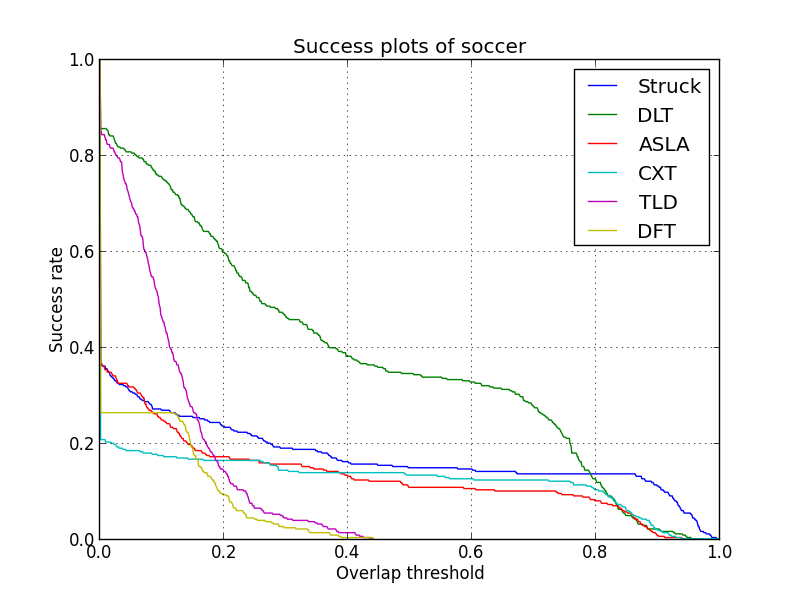
\includegraphics[width=200pt]{soccer}
    \caption{success rate score plot of soccer sequences}
    \label{fig:soccer}
\end{figure}

\textbf{CXT.} In this dataset, since the direction of person's face turned around and the condition surrounding the face changed dramatically, Supporters can't help to verify the location of the target. As for distracters, in the end of data there are many faces and the target is missing, so it's hard to find the right face.

\textbf{Struck.}
Soccer image has many pieces of ribbons which has stronger effect on Haar feature than human faces.~\ref{fig:struck_soccer}
\begin{figure}[hbt]
    \centering
    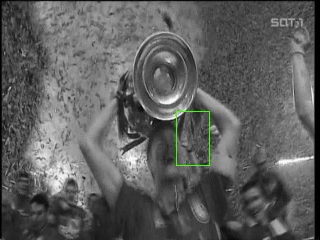
\includegraphics[width=140pt]{struck_soccer}
    \caption{Struck algorithm test on the soccer sequence, the backgourd has much more significant visual features than the player's face.}
    \label{fig:struck_soccer}
\end{figure}
\subsubsection{Subway}

\begin{figure}[hbt]
	\centering
    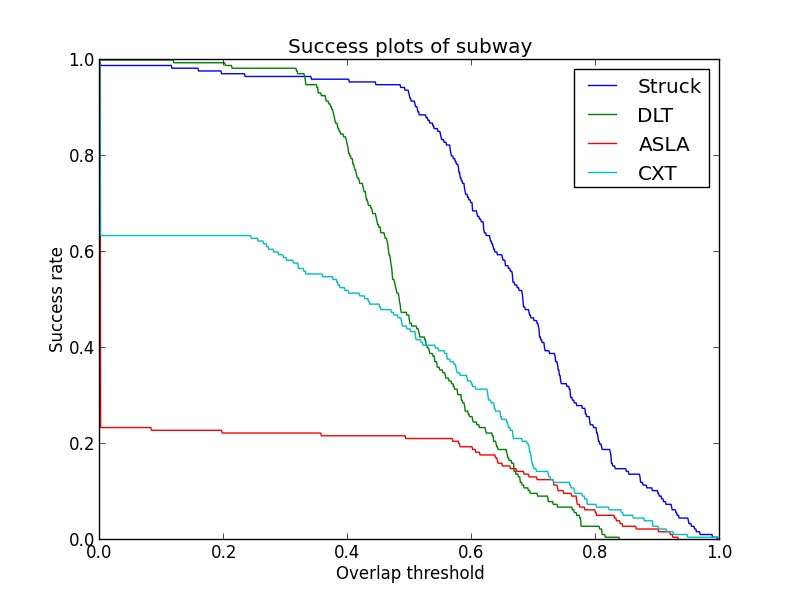
\includegraphics[width=200pt]{subway}
    \caption{success rate score plot of subway sequences}
    \label{fig:subway}
\end{figure}

\textbf{CXT.} It shows that Supports and Distracters don't do well in detecting the deformation.

\textbf{ALSA.} Because the tracker uses affine motion models, it handles well in scale variation (SV). That’s the explanation why ASLA performs best in Walking and Subway. 

\subsubsection{Suv}

\begin{figure}[hbt]
	\centering
    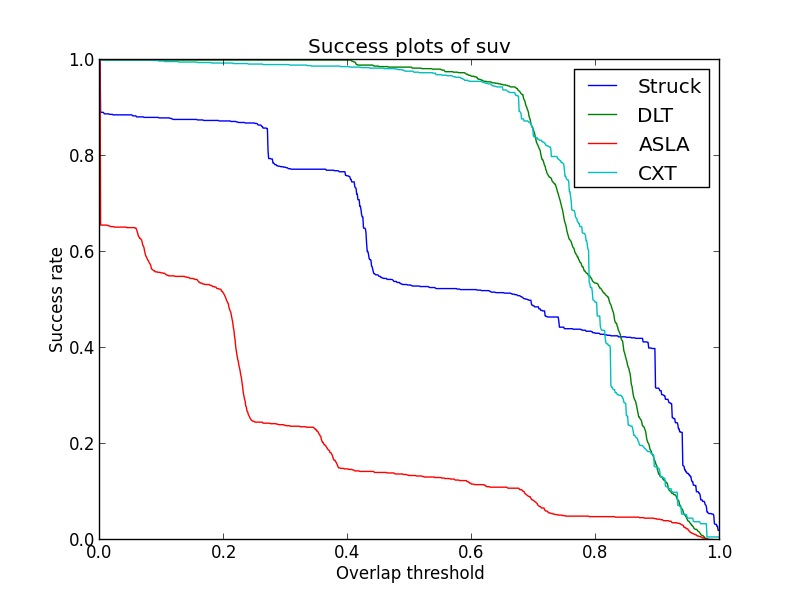
\includegraphics[width=200pt]{suv}
    \caption{success rate score plot of suv sequences}
    \label{fig:suv}
\end{figure}

\textbf{CXT.} In this sequence and sylvester sequence, tt shows that when the target is partially or fully occluded or some portion of the target leaves the view, CXT can find the target correctly. Since CXT uses the Supports which are local key-points around the object having motion correlation with the target in a short time span, CXT can find the location of target more precisely.

\textbf{ALSA.} The result in Suv suggests that structured learning and local sparse representations, adopted by ASLA, are effective in dealing with occlusions (OCC).

\textbf{Struck.} In SUV image, the SUV is occluded by trees and traffic lights, histogram of color feature is litter better than the Haar feature.
SUV's visual feature is also like the background road which is a reason for detected position stuck in the road.See Fig~\ref{fig:struck_suv}

\textbf{DFT.} The tracking window gradually diverges from the actual object: the suv car, since the occlusions of the car appears. See Fig~\ref{fig:dft_suv}

\begin{figure}[hbt]
	\centering
    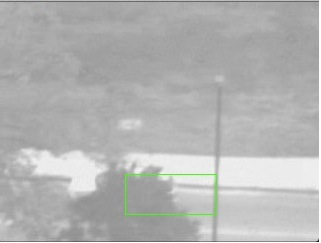
\includegraphics[width=140pt]{struck_suv}
    \caption{Struck algorithm test on the suv sequence. The tree has much more significant visual features than the suv on the left.}
    \label{fig:struck_suv}
\end{figure}

\begin{figure}[hbt]
	\centering
    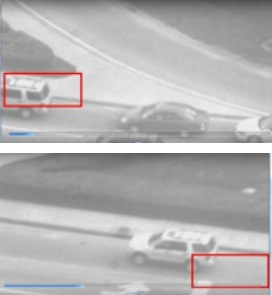
\includegraphics[width=140pt]{dft_suv}
    \caption{DFT algorithm test on the suv sequence. When suv leave the view, the predict bounding box will stay beside, which makes the right half of the box effects the tracker. The result becomes further worse when the time goes on, since more and more useless object are included in the window. Other algorithms like struck has the same situation.}
    \label{fig:dft_suv}
\end{figure}

\subsubsection{Sylvester}

\begin{figure}[hbt]
	\centering
    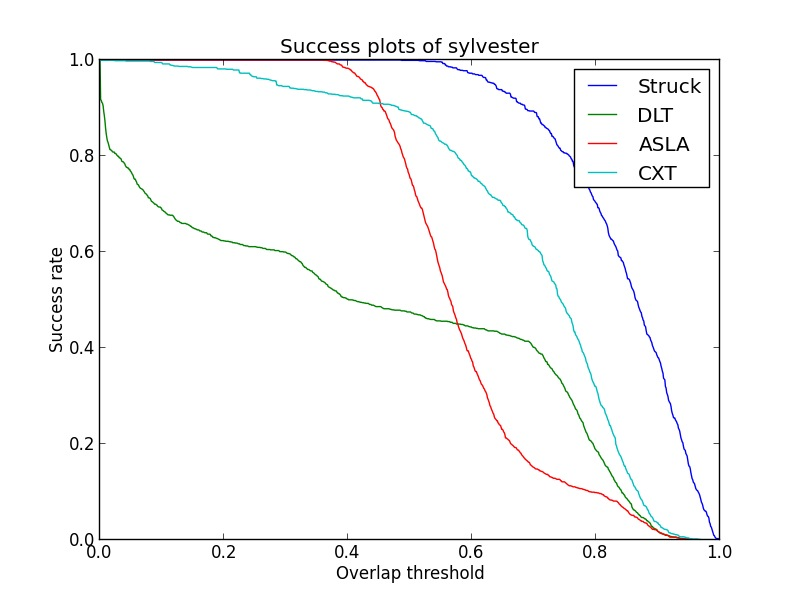
\includegraphics[width=200pt]{sylvester}
    \caption{success rate score plot of sylvester sequences}
    \label{fig:sylvester}
\end{figure}

\textbf{CXT.} It shows that illumination variation, in-plane rotation and out-of-plane rotation don't matter detection acutely. The reason might be Supports and Distracters that give more evidences to find the target and eliminate the wrong object.

\textbf{DFT.} We could learn that the window size will also diverge when be confronted with rotations, where the human change the orientations of the head of the toy dog.~\ref{fig:dtf_sylvester}
\begin{figure}[hbt]
	\centering
    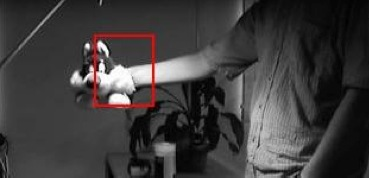
\includegraphics[width=140pt]{dtf_sylvester}
    \caption{DFT algorithm test on the suv sequence.}
    \label{fig:dtf_sylvester}
\end{figure}

\subsubsection{Tiger1}

In the tiger1 sequence, the target is a fast moving toy with motion blur.

\begin{figure}[hbt]
	\centering
    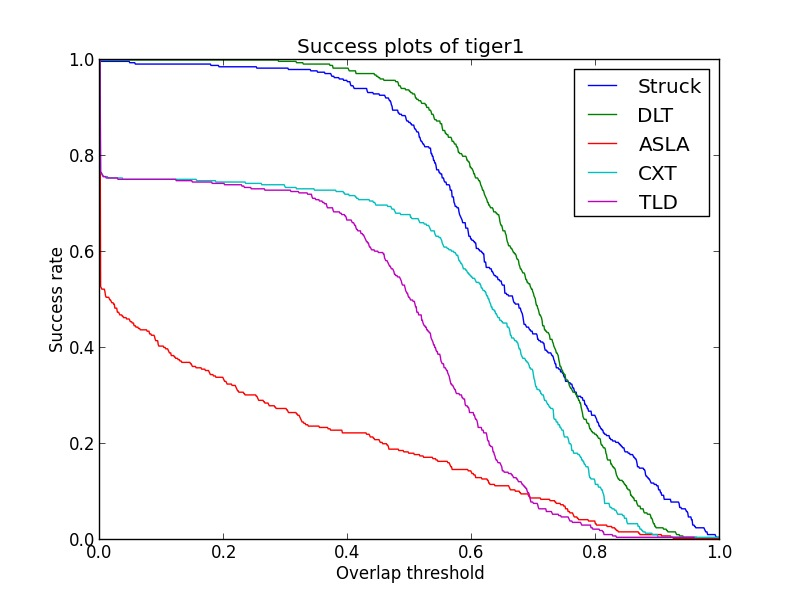
\includegraphics[width=200pt]{tiger1}
    \caption{success rate score plot of tiger1 sequences}
    \label{fig:tiger1}
\end{figure}

\textbf{CXT.} It shows that when the motion of the ground truth is fast and the target has a deformation, CXT can't detect the target. Because the condition changes dramatically, Supports and Distracters can't be calculated precisely. And they might not do well in detecting the deformation.

\textbf{DLT.} DLT with a higher value of x and y translation can track tiger1 successfully.

\subsubsection{Tiger2}

In the tiger1 sequence, the target is a fast moving toy with motion blur.

\begin{figure}[hbt]
	\centering
    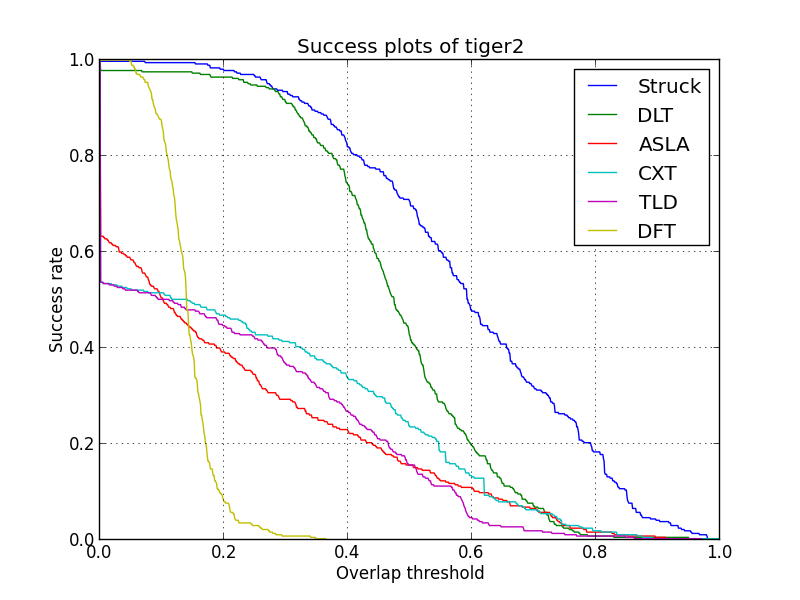
\includegraphics[width=200pt]{tiger2}
    \caption{success rate score plot of tiger2 sequences}
    \label{fig:tiger2}
\end{figure}

\textbf{CXT} It shows that when the motion of the ground truth is fast and the target has a deformation, CXT can't detect the target. Because the condition changes dramatically, Supports and Distracters can't be calculated precisely. And they might not do well in detecting the deformation.

\textbf{DLT} DLT with a higher value of x and y translation can track tiger1 successfully, while lost track of tiger2 in about frame 160. In the woman sequence, the woman is severely occluded several times by the parked cars. DLT tracker fails when the woman walks close to the car at about frame 130.

\subsubsection{Trellis}

In the trellis sequence, each tracker has to track a face in outdoor environments with a abrupt change of motion.

\begin{figure}[hbt]
	\centering
    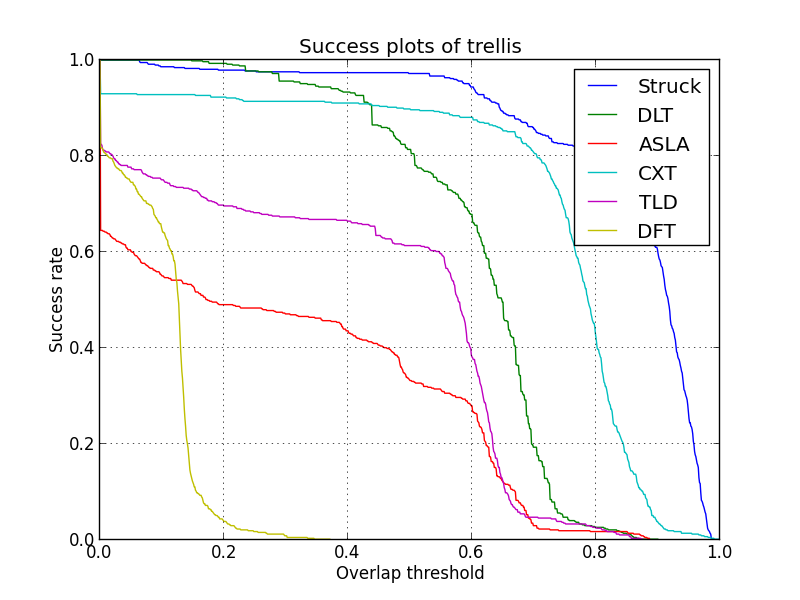
\includegraphics[width=200pt]{trellis}
    \caption{success rate score plot of trellis sequences}
    \label{fig:trellis}
\end{figure}

\textbf{CXT.} In this sequence and trellis, it shows that illumination variation, in-plane rotation and out-of-plane rotation don't matter detection acutely. The reason might be Supports and Distracters that give more evidences to find the target and eliminate the wrong object.

\subsubsection{Walking}

\begin{figure}[hbt]
	\centering
    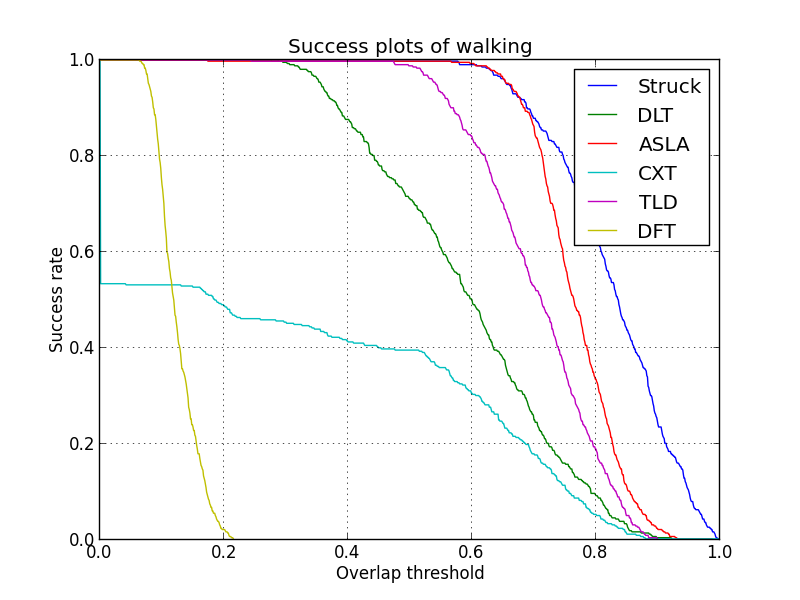
\includegraphics[width=200pt]{walking}
    \caption{success rate score plot of walking sequences}
    \label{fig:walking}
\end{figure}

\textbf{CXT} It shows that Supports and Distracters don't do well in detecting the deformation.

\textbf{ALSA.} While comparing the result in Walking with in Walking2, the tracker behaviors differently. We analysis that ASLA always fails in subset with some frames where the target is fully or partially obstruct by the similar. 

\subsubsection{Walking2}

\begin{figure}[hbt]
    \centering
    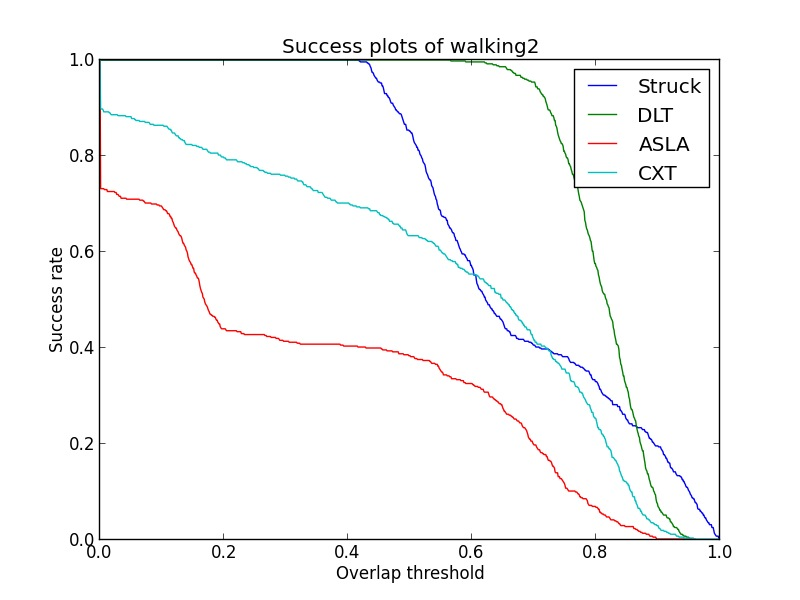
\includegraphics[width=200pt]{walking2}
    \caption{success rate score plot of walking2 sequences}
    \label{fig:walking2}
\end{figure}

\textbf{CXT.} It shows that Low Resolution might influence the detection. Since low resolution and occlusion, it will be hard to find appropriate Supports to find the target.

\subsubsection{Woman}

In the woman sequence, the woman is severely occluded several times by the parked cars.

\begin{figure}[hbt]
	\centering
	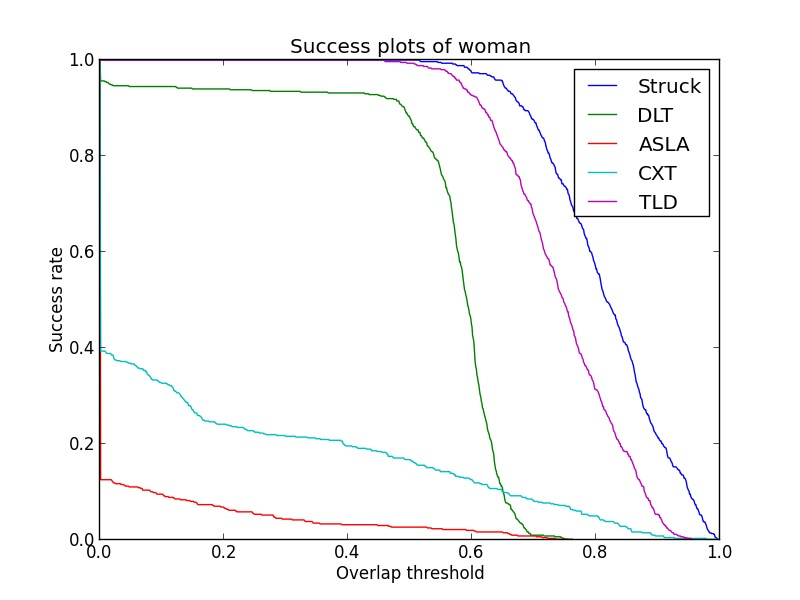
\includegraphics[width=200pt]{woman}
	\caption{success rate score plot of woman sequences}
	\label{fig:woman}
\end{figure}

\textbf{CXT.} The combination of Deformation, Motion Blur and Fast Motion make detection harder. The Supports and Distracters don't work better in these factors. Fast Motion makes it hard to detect the local key-points around the object having motion correlation with the target in a short time span. Deformation and Motion Blur seriously affects to find the target.

\textbf{DLT.} DLT tracker fails when the woman walks close to the car and the camera is rolling in. A dramatically change both of scale and occlusion is really hard to handle.

\subsection{Speed Analysis}

\begin{table}
	\centering
	\begin{tabular}{|c|c|l|} \hline
		Method & Implementation & FPS\\ \hline
		Struck & C & 9.3\\ \hline
		DLT & C \& MATLAB & 17.0\\ \hline
		CXT & C \& MATLAB & 15.3\\ \hline
		ASLA & C \& MATLAB & 8.5\\ \hline
		DFT & MATLAB & 4\\ \hline
		TLD & C \& MATLAB & 13.2\\ \hline
	\end{tabular}
	\caption{Comparison of average running time on 10 video sequences (in fps).}
	\label{table:time}
\end{table}

We also list the average running time of each algorithms of 10 sequence in detail in Table~\ref{table:time}. Thanks to advances of the GPU technology, DLT can achieve an average frame rate of 17 fps. While all algorithms we evaluated are sufficient for many real-time applications.

\section{Conclusions}
In this paper, we run massive amount of experiments to evaluate the performance of 6 selected tracking algorithms.
We use different image sequences to evaluate algorithms in different situations.
Each algorithm has its own better situation and worse situation.
Struck is good for slow moving objects which do not leave the view. And the target should better not have background clutters which can make the image feature significantly different.
Such as DLT is good at handling occlusion, while no so good at handling abrupt illumination changes.
ASLA perform well in images with occlusion and scale variation, but bad in sequeces with fast motion targets.
CXT is affected much by deformation and motion blur, but is able to track the target with in-plane and out-plane rotation.


\begin{thebibliography}{99}
\bibitem{struck}
S. Hare, A. Saffari, and P. H. S. Torr. Struck: Structured Output Tracking with Kernels. In ICCV, 2011.

\bibitem{shi1}
A. Adam, E. Rivlin, and I. Shimshoni. Robust fragments-based tracking using the integral histogram. In CVPR, 2006.

\bibitem{shi2}
B. Babenko, M.-H. Yang, and S. Belongie. Visual tracking with online multiple instance learning. In CVPR, 2009.

\bibitem{shi3}
J. Kwon and K. M. Lee. Visual tracking decomposition. In CVPR, 2010.

\bibitem{shi4}
D. Ross, J. Lim, R.-S. Lin, and M.-H. Yang. Incremental learning for robust visual tracking. IJCV, 77(1): 125141, 2008.

\bibitem{shi5}
J. Santner, C. Leistner, A. Saffari, T. Pock, and H. Bischof. Prost: Parallel robust online simple tracking. In CVPR, 2010.

\bibitem{shi6}
X. Mei and H. Ling. Robust visual tracking using L1 minimization. In ICCV, 2009.

\bibitem{shi7}
Z. Kalal, J. Matas, and K. Mikolajczyk. P-N learning: Bootstrapping binary classifiers by structural constraints. In CVPR, 2010.

\bibitem{dlt}
Wang, Naiyan, and Dit-Yan Yeung. Learning a Deep Compact Image Representation for Visual Tracking. Advances in Neural Information Processing Systems. 2013.

\bibitem{tiny}
Torralba, Antonio, Robert Fergus, and William T. Freeman. 80 million tiny images: A large data set for nonparametric object and scene recognition. Pattern Analysis and Machine Intelligence, IEEE Transactions on 30.11 (2008): 1958-1970.

\bibitem{benchmark}
Y.Wu, J. Lim, M.H. Y. Online Object Tracking: A Benchmark. In CVPR, 2013

\bibitem{asla}
X.Jia, H.Lu. M.H Yang, Visual Tracking via Adaptive Structural Local Sparse Appearance Model, In CVPR, 2012

\bibitem{tld}
Z. Kalal, J. Matas, and K. Mikolajczyk. P-N Learning: Bootstrapping Binary Classifiers by Structural Constraints. In CVPR, 2010.

\bibitem{cxt}
T. B. Dinh, N. Vo, and G. Medioni. Context Tracker: Exploring supporters and distracters in unconstrained environments. In CVPR, 2011.

\bibitem{dcmt}
A.Andriyenko, K.Schindler, S.Roth. Discrete-Continuous Optimization for Multi-Target Tracking. CVPR 2012.

\bibitem{rw1}
Y. Boykov, O. Veksler, and R. Zabih. Fast approximate energy minimization via graph cuts. PAMI, 23(11), 2001

\bibitem{rw2}
V. Kolmogorov. Convergent tree-reweighted message passing for energy minimization. PAMI, 28(10), 2006.

\bibitem{rw3}
V. Kolmogorov and R. Zabih. What energy functions can be minimized via graph cuts? PAMI, 26(2), 2004

\bibitem{rw4}
Z. Khan, T. Balch, and F. Dellaert. MCMC data association and sparse factorization updating for real time multitarget tracking with merged and multiple measurements. PAMI’06.

\bibitem{rw5}
S. Oh, S. Russell, and S. Sastry. Markov chain Monte Carlo data association for general multiple-target tracking problems. IEEE Conference on Decision and Control, 2004.

\bibitem{rw6}
B. Liu, J. Huang, L. Yang, and C. A. Kulikowski. Robust tracking using local sarse appearance model and k-selection. In CVPR, 2011.

\bibitem{rw7}
Z. Kalal, J. Matas, and K. Mikolajczyk. P-N learning: Bootstrapping binary classifiers by structural constraints. In CVPR, pages 49–56, 2010.

\bibitem{rw8}
Z. Kalal, J. Matas, and K. Mikolajczyk. Online learning of robust object detectors during unstable tracking. In OLCV, pages 1417–1424, 2009.

\bibitem{rw9}
I. Tsochantaridis, T. Joachims, T. Hofmann, and Y. Altun. Large Margin Methods for Structured and Interdependent Output Variables. JMLR, 6:1453–1484, Dec. 2005.

\bibitem{rw10}
A. Bordes, L. Bottou, P. Gallinari, and J. Weston. Solving multiclass support vector machines with LaRank. In Proc. ICML, 2007. 2, 4

\bibitem{rw11}
A. Bordes, N. Usunier, and L. Bottou. Sequence Labelling SVMs Trained in One Pass. In Proc. ECML-PKDD, 2008. 2, 4, 5

\bibitem{dataset}
\url{https://sites.google.com/site/trackerbenchmark/benchmarks/v10}

\end{thebibliography}

\end{document}
